\begin{name}
	{ÔN TẬP KIỂM TRA CUỐI HỌC KÌ 1}
	{TOÁN 10}
	{LỚP TOÁN THẦY PHÁT}
	{\thoigian}
\end{name}

\caulc
\Opensolutionfile{ans}[ans/10-CK1-Toan-tu-tam-De-3-Phan-1]

\begin{ex}
Trong các mệnh đề sau, mệnh đề nào \textbf{sai}?
\choice
{\True Số $1$ không là nghiệm phương trình $x^2-2x+1=0$}
{$\exists n \in \mathbb{N}, n^2=100$}
{Hình thoi có hai đường chéo vuông góc nhau}
{Tập rỗng là tập con của mọi tập hợp}
\loigiai{
	Phương trình $x^2-2x+1=0$ có nghiệm $x=1$.
}
\end{ex}

\begin{ex}
Cho $A=\left(\dfrac{3}{4}; 5\right]$, $B=[2; +\infty)$. Tập hợp $A \cup B$ là
	\choice
	{$\left(\dfrac{3}{4}; 5\right]$}
	{\True $\left(\dfrac{3}{4}; +\infty\right)$}
	{$[2; 5]$}
	{$[2; +\infty)$}
	\loigiai{
	Ta có $A \cup B = \left(\dfrac{3}{4}; 5\right] \cup [2; +\infty) = \left(\dfrac{3}{4}; +\infty\right)$.
	}
\end{ex}

\begin{ex}%[0D2N2-1]
Cặp số nào sau đây là nghiệm của bất phương trình $(x-2)+2(y+1)<4$?
	\choice
	{$(2;1)$}
	{\True $(-3;-1)$}
	{$(0;2)$}
	{$(1;2)$}
	\loigiai{
	Thay các cặp số vào bất phương trình ta thấy chỉ có cặp số $(-3;-1)$ thoả mãn.
	}
\end{ex}

\begin{ex}%[0H4N1-1]
Cho góc $a$ thoả mãn $0^\circ<a<180^\circ$. Trong các mệnh đề sau, mệnh đề nào \textbf{đúng}? 
	\choice
	{\True $\sin a \in (0;1]$}
	{$\cos a \in [0;1]$}
	{$\tan a \in (-\infty;0)$}
	{$\cot a \in (-\infty;0)$}
	\loigiai{
		Vì $0^\circ<a<180^\circ$ nên $\sin a \in (0;1]$, $\cos a \in (-1;1)$, $\tan a \in \mathbb{R}$ (với $a \neq 90^\circ$) và $\cot a \in \mathbb{R}$.
	}
\end{ex}

\begin{ex}%[0H4N3-1]
Cho tam giác $ABC$ với $AB=c$, $AC=b$, $BC=a$ có diện tích $S$ và nửa chu vi $p$. Trong các mệnh đề sau, mệnh đề nào \textbf{đúng}?
	\choice
	{$S=ab\sin C$}
	{\True $S=\sqrt{p(p-a)(p-b)(p-c)}$}
	{$S=\dfrac{1}{2}ac\cos B$}
	{$p=\dfrac{abc}{2S}$}
	\loigiai{
		Ta có $S=\sqrt{p(p-a)(p-b)(p-c)}$ (công thức Heron).
	}
\end{ex}

\begin{ex}%[0H5N1-1]
Hai vectơ bằng nhau là hai vectơ có
	\choice
	{cùng độ dài}
	{cùng độ dài và cùng phương}
	{\True cùng độ dài, cùng hướng}
	{cùng độ dài và ngược hướng}
	\loigiai{
		Hai vectơ $\overrightarrow{a}$ và $\overrightarrow{b}$ bằng nhau khi và chỉ khi chúng có cùng độ dài và cùng hướng.
	}
\end{ex}

\begin{ex}%[0H5H2-4]
Cho hình thang vuông $ABCD$ có hai đáy $AB$ và $CD$ vuông góc với cạnh bên $AD$. Biết $AB=6$, $CD=10$ và $\widehat{BCD}=45^\circ$. Tính độ dài vectơ $\overrightarrow{AD}+\overrightarrow{BC}$.
\choice
{$6\sqrt{2}$}
{\True $4\sqrt{5}$}
{$6\sqrt{3}$}
{$4\sqrt{2}$}
\loigiai{
\immini{Gọi $E$ là đỉnh thứ tư của hình bình hành $ABCE$. Suy ra $\widehat{BCD}=\widehat{AED}=45^\circ$ và $ED=CD-AB=4$.\\
Khi đó $\overrightarrow{AD}+\overrightarrow{BC}=\overrightarrow{AD}+\overrightarrow{AE}=\overrightarrow{AF}$ (với $F$ là đỉnh còn lại của hình bình hành $AEFD$).\\
Ta có $AF=\sqrt{(2AD)^2+ED^2}=\sqrt{(2\cdot 4)^2+4^2}=4\sqrt{5}$.}
{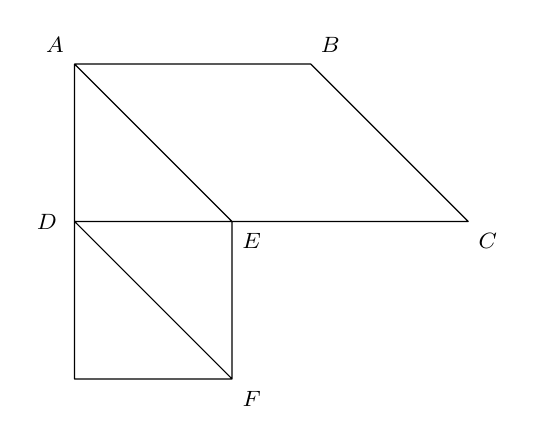
\begin{tikzpicture}[scale=0.5, font=\footnotesize, line join=round, line cap=round]
	\path
	(0,0) coordinate (A)
	(6,0) coordinate (B)
	(10,-4) coordinate (C)
	(0,-4) coordinate (D)
	(4,-4) coordinate (E)
	(4,-8) coordinate (F);
	\draw (A)--(B)--(C)--(D)--cycle (A)--(E)--(F)--(D) (F)-|(D);
	\foreach \d/\g in {A/135,B/45,C/-45,D/180,E/-45,F/-45} \draw[fill=black] (\d) node[shift={(\g:10pt)}]{$\d$} ;
	\end{tikzpicture}}
}
\end{ex}
\begin{ex}%[0-HK1-KN-1-PhanDinhPhung-HaNoi-2324]%[VN-MT-6, VM019]%[0H9H1-1]
Trong mặt phẳng tọa độ $Oxy$, cho $\overrightarrow{OM}=\overrightarrow{i}+2\overrightarrow{j}$, $\overrightarrow{ON}=2\overrightarrow{i}$. Tìm tọa độ vectơ $\overrightarrow{MN}$.
\choice
{\True $\overrightarrow{MN}=(1;-2)$}
{$\overrightarrow{MN}=(1;2)$}
{$\overrightarrow{MN}=(-1;-2)$}
{$\overrightarrow{MN}=(-1;2)$}
\loigiai{
Tọa độ điểm $M(1;2)$ và $N(2;0)$ nên $\overrightarrow{MN}=(1;-2)$.
}
\end{ex}

\begin{ex}%[0D8N1-2]%[Dự án soạn đề kiểm tra Toán 10 HKII NH24-25- Mui Doan]%[CTST_0_OTHK2-De02]
Một lớp học có $6$ em học sinh ra ứng cử chức vụ lớp trưởng, lớp phó học tập và thủ quỹ của lớp. Hỏi có bao nhiêu cách chọn lớp trưởng, lớp phó học tập và thủ quỹ?
\choice
{$6$}
{$15$}
{$4$}
{\True $120$}
\loigiai{
Có $6$ cách chọn lớp trưởng, $5$ cách chọn lớp phó học tập, và $4$ cách chọn thủ quỹ.\\
Theo quy tắc nhân, số cách thực hiện là $6 \cdot 5 \cdot 4 = 120$ (cách).
}
\end{ex}

\begin{ex}%[Đề chuẩn hóa Toán 11]%[Nguyễn Trung Kiên]%[0D8N2-1]
Tính số chỉnh hợp chập $4$ của $7$ phần tử.
\choice
{$35$}
{\True  $840$}
{$336$}
{$56$}
\loigiai{
Số chỉnh hợp chập $4$ của $7$ phần tử là $\mathrm{A}_7^4=\dfrac{7!}{(7-4)!}=840$.
}
\end{ex}

\begin{ex}%[0D8N3-1]
Hãy chọn khẳng định đúng?
\choice
{$(a+b)^4=a^4+2a^3b+3a^2b^2+4ab^3+b^4$}
{$(a+b)^4=a^4+b^4$}
{$(a+b)^4=a^4+a^3b+a^2b^2+ab^3+b^4$}
{\True $(a+b)^4=a^4+4a^3b+6a^2b^2+4ab^3+b^4$}
\loigiai{
Ta có $(a+b)^4=a^4+4a^3b+6a^2b^2+4ab^3+b^4$.
}
\end{ex}

\begin{ex}%[0D8H2-5]
Có $4$ bì thư khác nhau và $7$ tem thư khác nhau. Bạn An muốn gửi thư cho $4$ người bạn của mình. Hỏi có bao nhiêu cách gửi, biết rằng mỗi bì thư chỉ dán một tem thư.
\choice
{\True $20\,160$}
{$840$}
{$35$}
{$12\,980$}
\loigiai{
\begin{itemize}
\item Chọn $4$ tem thư dán vào $4$ bì thư có $\mathrm{A}_7^4=840$ cách.
\item Gửi $4$ bì thư đã dán tem thư cho $4$ người bạn có $4!=24$ cách.
\end{itemize}
Theo quy tắc nhân ta có $840 \cdot 24 = 20\,160$ cách.
}
\end{ex}
\Closesolutionfile{ans}
% \indapan{6}{ans/10-CK1-Toan-tu-tam-De-3-Phan-1}\

\cauds
\Opensolutionfile{ans}[ans/10-CK1-ToanTuTam-Phan-2]
\begin{ex}%[0D8H2-5]
Cho các số $1;2;3;4;5;6$. Xét tính đúng sai của các khẳng định sau.
\choiceTF[t]
{\True  Có $720$ số có $6$ chữ số được lập từ các chữ số đã cho}
{Có thể lập được $1\,296$ số có $4$ chữ số khác nhau từ các chữ số đã cho}
{\True Số cách chọn $4$ số từ các số đã cho là $15$ cách}
{Số cách chọn $4$ số, trong đó luôn có số $2$ từ các số đã cho là $20$ cách}
\loigiai{
\begin{itemchoice}
\itemch \textbf{Đúng}. Có $6!=720$ số có $6$ chữ số được lập từ các chữ số đã cho.
\itemch \textbf{Sai}. Có $\mathrm{A}_{6}^4=120$ số có $4$ chữ số khác nhau được lập từ các chữ số đã cho.
\itemch \textbf{Đúng}. Số cách chọn $4$ số từ các số đã cho là $\mathrm{C}_{6}^4=15$.
\itemch \textbf{Sai}.
Số cách chọn $4$ số, trong đó luôn có số $2$ là $\mathrm{C}_{5}^3=10$.
\end{itemchoice}
}

\end{ex}
\begin{ex}%[0H9H2-1]%[KNTT - Lớp 10 - Ôn tập cuối học kì 1 - Đề 6]%[Nguyễn Hoài Nam]
Cho ba điểm $A(-2;5)$, $B(-4;-2)$; $C(1;5)$.
\choiceTF
{Tọa độ véc-tơ $\overrightarrow{u}=2\overrightarrow{AB}+\overrightarrow{AC}$ là $(1;14)$}
{\True Ba điểm $A$, $B$, $C$ tạo thành một tam giác}
{\True Tích vô hướng của hai véc-tơ $\overrightarrow{AB}$ và $\overrightarrow{AC}$ bằng $-6$}
{Gọi $G$ là trọng tâm tam giác $ABC$ ta có \ $\cos{(\overrightarrow{AB};\overrightarrow{CG})\approx 2{,}84}$}
\loigiai{
\begin{itemchoice}
\itemch Ta có $\overrightarrow{AB}=(-2;-7);\ \overrightarrow{AC}=(3;0)\Rightarrow \overrightarrow{u}=2\cdot \overrightarrow{AB}+\overrightarrow{AC}=2(-2;-7)+(3;0)=(-1;-14)$.
\itemch Ta có $\overrightarrow{AB}=(-2;-7);\ \overrightarrow{AC}=(3;0\Rightarrow\dfrac{3}{-2}\ne \dfrac{0}{-7}$. Suy ra $\overrightarrow{AB}$ và $\overrightarrow{AC }$ không cùng phương. Suy ra ba điểm $A$, $B$, $C$ lập thành một tam giác.
\itemch Ta có $\overrightarrow{AB}=(-2;-7);\overrightarrow{AC}=(3;0
)\Rightarrow\overrightarrow{AB}\cdot\overrightarrow{AC}=-2\cdot 3+0\cdot (-7)=-6$.
\itemch Với $G$ là trọng tâm tam giác $ABC$.\\
Khi đó $\heva{&x_G=\dfrac{-2+4+1}{3}=\dfrac{-5}{3}\\&y_G=\dfrac{5-2+5}{3}=\dfrac{8}{3}}$.\\
Suy ra $G\left(-\dfrac{5}{3};\dfrac{8}{3}.\right)$\\
Ta có $\overrightarrow{CG}=\left(-\dfrac{8}{3};-\dfrac{7}{3}\right)\Rightarrow \cos{(\overrightarrow{AB}, \overrightarrow {CG})}\approx 0{,}84$.
\end{itemchoice}
}
\end{ex}

\Closesolutionfile{ans}
% \indapan{3}{ans/10-CK1-ToanTuTam-Phan-2}

\caukq
%\Opensolutionfile{ans}[ans/CK1 10-CK1-Toan-tu-tam-De-3]
\Opensolutionfile{ans}[ans/CK1-10-CK1-Toan-tu-tam-De-3]

\begin{ex}%[0-HK1-CT-8-HoangHoaTham-HCM-2324]%[VN-MT-6, Trịnh Văn Cảnh]%[0D1H3-3]
Cho hai tập $A=[0;5]$; $B=(2a; 3a+1]$. Có bao nhiêu số tự nhiên $a$ để $A \cap B \neq \varnothing$?\par
\shortans[]{$3$} %Chuẩn hóa ko quá 4 ký tự
\loigiai{Ta có $A \cap B \neq \varnothing \Leftrightarrow\heva{&2a<3a+1\\ &\hoac{&0<2a<5\\ &0\leq 3a+1\leq 5\\&2a\leq 0<5\leq 3a+1}} \Leftrightarrow-\dfrac{1}{3}\leq a<\dfrac{5}{2}$.\\ Vì $a$ là số tự nhiên nên $a\in\{0;1;2\}$. Do đó có $3$ giá trị của $a$ thỏa mãn.}
\end{ex}

\begin{ex}%[Mức độ 2]%[0D2H1-2]%[Đỗ Đường Hiếu]
\immini{Phần nửa mặt phẳng không bị gạch (không kể đường thẳng $d$) ở hình vẽ sau là miền nghiệm của bất phương trình $x+m y>n$. Giá tri của biểu thức $S=5 m+n$ bằng bao nhiêu?}{
\begin{tikzpicture}[scale=0.8, font=\footnotesize, line join=round, line cap=round, >=stealth]
\draw[->] (-3,0) -- (3.5,0)node[above]{$x$};
\foreach \x in {2}
\draw[shift={(\x,0)},color=black] (0pt,2pt) -- (0pt,-2pt) node[above right] {\footnotesize $\x$};
\draw[->,color=black] (0,-1) -- (0,3.5)node[right]{$y$};
\foreach \y in {2}
\draw[shift={(0,\y)},color=black] (2pt,0pt) -- (-2pt,0pt) node[above right] {\footnotesize $\y$};
\node[below left] at (0,0) {$O$};
\clip(-3,-1) rectangle (3.5,3.5);
\fill[pattern=north east lines] (-3,3) -- (-1,3) -- (3,-1) -- (-3,-1) -- cycle;
\draw[line width=1.2pt,smooth,samples=100,domain=-1:4] plot(\x,{2-(\x)});
\end{tikzpicture}
}
\shortans{$7$}
\loigiai{
Đường thẳng $d\colon y=ax+b$. Theo hình vẽ, $d$ đi qua hai điểm $(0;2)$ và $(2;0)$ nên ta có hệ:
\[\heva{&a\cdot 0+b=2\\&a\cdot 2+b=0}\Leftrightarrow \heva{&a=-1\\&b=2.}\]
Vậy $d\colon y=-x+2 \Leftrightarrow x+y=2$.
Do gốc $O(0;0)$ không thuộc miền nghiệm của hệ nên ta có bất phương trình phải tìm là $x+y>2$. Vậy ta có $m=1, n=2 \Rightarrow S=7$.
}
\end{ex}

\begin{ex}%[0H4V3-2]
	\immini[thm]{Bạn An đứng ở sân thượng của tòa nhà và quan sát chiếc diều, nhận thấy góc giữa phương nhìn từ mắt của An tới chiếc diều và phương nằm ngang là $\alpha=50^\circ$. Khoảng cách từ sân thượng tòa nhà tới mắt của An là $1{,}7$ m. Cùng lúc đó, ở dưới chân tòa nhà theo phương thẳng đứng với vị trí của An, bạn Bình cũng quan sát chiếc diều đó và thấy góc giữa phương nhìn từ mắt của Bình tới chiếc diều và phương nằm ngang là $\beta=75^\circ$. Khoảng cách từ mặt đất tới mắt của Bình là $1{,}6$ m. Biết chiều cao của tòa nhà là $h=22$ m (hình vẽ).
		Hỏi chiếc diều ở vị trí cách mặt đất bao nhiêu mét (các phép toán làm tròn kết quả đến hàng phần chục)?}
	{\begin{tikzpicture}[scale=0.8, font=\footnotesize, line join=round, line cap=round, >=stealth,]
			\begin{scope}[shift=({0.2,0})]
				% Con dieu
				\filldraw[fill=orange!50,draw=brown] (3.5,5)--(2.8,4.9)--(2.6,5.5)--(3.2,5.6)--cycle;
				\draw[color=brown] (3.5,5)--(2.6,5.5) (2.8,4.9)--(3.2,5.6);
				\draw[line width=0.5mm,rounded corners,color=orange] (3.5,5)--(3.7,5.1)--(4,4.9)--(4.4,5.1) (3.5,5)--(3.6,4.8)--(3.9,4.9)--(4.5,5);
			\end{scope}
			% Cac chi tiet con lai
			\draw (0,0)--(2,0)--(2,4.2)--(0,4.2)--(0,0);
			\draw (1,0)--(1,4.2);
			\foreach \x in {0.7,1.4,...,3.5}{
				\draw (0,\x)--(2,\x);
			}
			\path
			(2,4.55) coordinate (A)
			(3.2,4.55) coordinate (A')
			(2,0.35) coordinate (B)
			(3.2,0.35) coordinate (B')
			(3.2,5.25) coordinate (C)
			;
			\draw (3.2,0)--(2,0)--(A)--(C)--(B);
			\draw[dashed] (C)--(3.2,0) (A)--(A') (B)--(B');
			\foreach \d/\g in {} \fill (\d)node[shift={(\g:0.3)}]{$\d$} circle(1pt);
			\pic[draw,angle radius=4mm,angle eccentricity=1.5] {angle = A'--A--C};
			\pic[draw,angle radius=4mm,angle eccentricity=1.5] {angle = B'--B--C};
			\pic[draw,angle radius=5mm,angle eccentricity=1.5] {angle = B'--B--C};
			\fill (0,1.4)node[shift={(180:0.3)}]{$h$};
			\fill (A)node[shift={(13:0.65)}]{$\alpha$};
			\fill (B)node[shift={(40:0.75)}]{$\beta$};
	\end{tikzpicture}}
	\par
	\shortans[]{34{,}1}
	\loigiai{
		\begin{center}
			\begin{tikzpicture}[scale=0.8, font=\footnotesize, line join=round, line cap=round, >=stealth,]
				% Cac chi tiet con lai
				\draw (0,0)--(2,0)--(2,4.2)--(0,4.2)--(0,0);
				\draw (1,0)--(1,4.2);
				\foreach \x in {0.7,1.4,...,3.5}{
					\draw (0,\x)--(2,\x);
				}
				\path
				(2,4.55) coordinate (N)
				(3.2,4.55) coordinate (A')
				(2,0.35) coordinate (M)
				(3.2,0.35) coordinate (B')
				(3.2,5.25) coordinate (D)
				;
				\draw (3.2,0)--(2,0)--(N)--(D)--(M);
				\draw[dashed] (D)--(3.2,0) (N)--(A') (M)--(B');
				\foreach \d/\g in {N/180,M/180} \fill (\d)node[shift={(\g:0.3)}]{$\d$} circle(1pt);
				\pic[draw,angle radius=4mm,angle eccentricity=1.5] {angle = A'--A--C};
				\pic[draw,angle radius=4mm,angle eccentricity=1.5] {angle = B'--B--C};
				\pic[draw,angle radius=5mm,angle eccentricity=1.5] {angle = B'--B--C};
				\fill (0,1.4) node[shift={(180:0.3)}]{$h$};
				\fill (A) circle (1.5pt) node[shift={(13:0.65)}]{$\alpha$};
				\fill (B) circle (1.5pt) node[shift={(40:0.75)}]{$\beta$};
				\fill (C) circle (1.5pt) node[shift={(90:0.2)}]{$D$};
				\fill (B') circle (1.5pt) node[shift={(0:0.3)}]{$H$};
				\fill (3.2,4.55) circle (1.5pt) node[shift={(-45:0.3)}]{$K$};
				\fill (3.2,0) circle (1.5pt) node[shift={(-90:0.3)}]{$E$};
			\end{tikzpicture}
		\end{center}
		Đặt tên các điểm như hình vẽ với $M$, $N$ lần lượt là vị trí mắt của Bình, An. Ta có $MN=22{,}1$\,(m).\\ 
		Xét tam giác $MND$ có\\ $\widehat{MND}=90^\circ+50^\circ=140^\circ$, $\widehat{NMD}=90^\circ-75^\circ=15^\circ$, $\widehat{MDN}=180^\circ-140^\circ-15^\circ=25^\circ$.\\
		Áp dụng định lí sin cho tam giác $MND$ ta có $\dfrac{MD}{\sin N}=\dfrac{ND}{\sin M}=\dfrac{MN}{\sin D}$.\\ 
		Suy ra $MD=\dfrac{MN\cdot\sin N}{\sin D}=\dfrac{22{,}1\cdot \sin 140^{^\circ}}{\sin 25^{^\circ}} \approx 33{,}6$\,(m).\\ Xét tam giác $MHD$ vuông tại $H$, ta có
		$HD=MD\cdot \sin 75^\circ\approx 33{,}6\cdot \sin 75^\circ=32{,}5$\,(m).\\
		Do đó $DE\approx 1{,}6+32{,}5=34{,}1$\,(m).\\
		Vậy chiếc diều ở vị trí cách mặt đất khoảng $34{,}1$\,(m).
	}
\end{ex}
\begin{ex}%[0H9H1-1]
Trong mặt phẳng tọa độ $Oxy$, cho tam giác $ABC$ với $A(-2;0)$, $B(5;-4)$, $C(-5;1)$. Gọi $D(m-5;n+7)$ là một điểm sao cho tứ giác $ABCD$ là hình bình hành. Giá trị biểu thức $A=m+n$ bằng bao nhiêu?
\par
\shortans{$-9$}
\loigiai{
Ta có $\heva{&\overrightarrow{AB}=(7;-4)\\&\overrightarrow{DC}=(-m;-n-6).}$\\
Để tứ giác $ABCD$ là hình bình hành thì $\overrightarrow{AB}=\overrightarrow{DC}\Leftrightarrow\heva{&-m=7\\&-n-6=-4}\Leftrightarrow\heva{&m=-7\\&n=-2.}$\\
Vậy tổng $m+n=-7+(-2)=-9$.
}
\end{ex}
\TL

\begin{ex}%[0H5V2-6]
	\immini[thm]{Cho hai lực $\overrightarrow{F}_1=\overrightarrow{OA}$, $\overrightarrow{F}_2=\overrightarrow{OB}$ cùng tác động vào một vật tại điểm $O$. Cường độ hai lực $\overrightarrow{F}_1$, $\overrightarrow{F}_2$ lần lượt là $34$ N và $134$ N. Góc $\widehat{AOB}=120^\circ$. Tính cường độ của lực tổng hợp tác động vào vật. (làm tròn đến hàng đơn vị)}
	{\begin{tikzpicture}[scale=1, font=\footnotesize, line join=round, line cap=round, >=stealth,declare function={a=3; b=5; goc=-60; }]
			\path
			(0,0) coordinate (B)
			(a,0) coordinate (D)
			(goc:b) coordinate (O)
			($(D)+(O)$) coordinate (A);
			\draw (B)--(D)--(A)--(O)--cycle;
			\draw[->=stealth] (O)--(A);
			\draw[->=stealth] (O)--(B);
			\draw[->=stealth] (O)--(D);
			\foreach \x/\y/\z in {A/O/B}{
				\path (\y) pic[draw,angle radius=15pt,right,angle eccentricity=1.2,"$120^\circ$"]{angle = \x--\y--\z};
			}
			\foreach \t/\g in {A/-90,B/90,O/-90,D/90}{
				\draw[fill=white] (\t) circle (1pt) node[shift={(\g:9pt)},font=\scriptsize]{$ \t $};
			}
	\end{tikzpicture}}
	% \par
	% \shortans[]{121}
	\loigiai{
		Gọi $\overrightarrow{F}=\overrightarrow{F}_1+ \overrightarrow{F}_2$ là lực tổng hợp cần tìm.\\
		Dựng hình bình hành $OADB$. Ta có $\widehat{OAD}=180^\circ-\widehat{AOB}=60^\circ$.\\
		Khi đó cường độ của lực tổng hợp tác động vào vật là
		\allowdisplaybreaks
		\begin{eqnarray*}
			\left|\overrightarrow{F}\right|=\left|\overrightarrow{OA}+ \overrightarrow{OB}\right|&=&\left|\overrightarrow{OD}\right|\\
			&=&\sqrt{OA^2+AD^2-2\cdot OA\cdot AD\cdot\cos \widehat{OAD}}\\
			&=&\sqrt{34^2+134^2-2\cdot 34\cdot 134\cdot\cos 60^\circ}=2\sqrt{3\,639}\approx 121~ \text{N}.
		\end{eqnarray*}
	}
\end{ex}

\begin{ex}%[De-chuan-hoa-so-16]%[Mui Doan]%[0H9V1-6]
Để kéo đường dây điện băng qua một cái hố hình chữ nhật $ABCD$ với độ dài $AB=140$ m, $AD=50$ m. Người ta dự định làm $5$ cột điện liên tiếp thẳng hàng và cách đều nhau. Cột thứ nhất nằm trên bờ $AB$ và cách đỉnh $A$ một khoảng bằng $10$ m. Cột thứ năm nằm trên bờ $CD$ và cách đỉnh $C$ một khoảng bằng $30$ m. Tính khoảng cách từ cột thứ tư đến bờ $AD$.
% \shortans[]{$85$}
\loigiai{
\immini{
Chọn hệ trục tọa độ như hình vẽ với $A(0;0)$, $B(140;0)$, $C(104;50)$, $D(0;50)$. Chọn vị trí $5$ cột điện ở $C_1$, $C_2$, $C_3$, $C_4$, $C_5$ như hình vẽ. Vì $C_1$ thuộc $AB$ và cách $A$ một khoảng cách bằng $10$m nên $C_1(10;0)$. Vì $C_5\in BD$ và cách $C$ một đoạn bằng $30$m nên $C_5(110;50)$.\\
}
{
\begin{tikzpicture}[scale=0.8,>=stealth, font=\footnotesize, line join=round, line cap=round]
\def\xmin{-1} \def\xmax{6}  \def\ymin{-1}  \def\ymax{3}
%\draw[color=gray!50,dashed] (\xmin,\ymin) grid (\xmax,\ymax);
\draw[->] (\xmin,0)--(\xmax,0) node [below]{$x$};
\draw[->] (0,\ymin)--(0,\ymax) node [left]{$y$};
\clip (\xmin,\ymin) rectangle (\xmax,\ymax);
%%%%
\path (0,0) coordinate (A)
(5,0) coordinate (B)
(0,2) coordinate (D)
(0.5,0) coordinate (C_1)
(5,2) coordinate (C)
(3.5,2) coordinate (C_5)
($(C_1)!1/4!(C_5)$) coordinate (C_2)
($(C_1)!2/4!(C_5)$) coordinate (C_3)
($(C_1)!3/4!(C_5)$) coordinate (C_4)
;
\foreach \t/\g in {A/120,B/-90,C/90,D/180,C_1/-90,C_5/90,C_2/160,C_3/160,C_4/160}{
\draw[fill=black] (\t) circle (1pt) node[shift={(\g:7pt)},font=\scriptsize]{$ \t $};
}
\draw (A)--(B)--(C)--(D) (C_1)--(C_5);
\end{tikzpicture}
}
\noindent Ta có $\overrightarrow{C_1C_4}=\dfrac{3}{4}\overrightarrow{C_1C_5}\Leftrightarrow 4\overrightarrow{OC_4}-4\overrightarrow{OC_1}=3\overrightarrow{OC_5}-3\overrightarrow{OC_1}\Leftrightarrow \overrightarrow{OC_4}=\dfrac{1}{4}\overrightarrow{OC_1}+\dfrac{3}{4}\overrightarrow{OC_5}.$\\ Suy ra $C_4(85;37{,}5)$, do đó $AD$ cách cột điện thứ $4$ cách bờ $AD$ một khoảng bằng $85$ m.
}
\end{ex}
\begin{ex}%[0D8C2-3]
Từ các số $0$, $1$, $2$, $3$, $4$, $5$, $6$, $7$, $8$ có thể lập được bao nhiêu số tự nhiên có $5$ chữ số khác nhau sao cho luôn có mặt ba chữ số $0$, $1$, $2$ và ba chữ số này luôn phải đứng cạnh nhau?
% \shortans[oly]{$480$}
\loigiai{Số tự nhiên có $5$ chữ số khác nhau cần lập có dạng $\overline{abcde}$.\\
Chọn $1$ trong $3$ vị trí kề nhau trong các vị trí $abc,bcd,cde$ có $3$ cách.\\
Xếp $3$ chữ số $0,1,2$ vào $3$ vị trí kề nhau có $3!$ cách. \\
Chọn $2$ trong $6$ số $\{3,4,5,6,7,8\}$ xếp vào $2$ vị trí còn lại có $\mathrm{A}_6^2$ cách.\\
Vậy có $3 \cdot 3! \cdot \mathrm{A}_6^2 =540$ số.\\
Trong các số trên sẽ có các số có dạng $\overline{0bcde}$.\\
Xếp $2$ số $1,2$ vào các vị trí $b,c$ có $2!$ cách.\\
Chọn $2$ trong $6$ số $\{3,4,5,6,7,8\}$ xếp vào $2$ vị trí còn lại có $\mathrm{A}_6^2$ cách.\\
Vậy có $2! \cdot \mathrm{A}_6^2 =60$ số có dạng $\overline{0bcde}$ trong $540$ số đã lập ở trên.\\
Do đó số các số tự nhiên có $5$ chữ số sao cho luôn có mặt ba chữ số $0,1,2$ và ba chữ số này luôn phải đứng cạnh nhau là $540-60=480$ số.
}
\end{ex}
\Closesolutionfile{ans}
% \indapan{6}{ans/CK1-10-CK1-Toan-tu-tam-De-3}